\section{Learning MPIs}\label{sec:learning-mpis} 

Some of the major challenges in high-quality novel view synthesis include synthesizing pixels occluded in one or more of the provided views, disentangling and localizing ambiguous pixels at/near the boundaries of foreground and background objects, localizing pixels at transparent, translucent, reflective, or texture-less surfaces, etc. Moreover, whereas interpolating novel views at desired viewpoints lying within the convex hull of given viewpoints is easier to achieve than extrapolating significantly beyond the baselines (distances between camera centers) of input views, these challenges can emerge in either case. So far, it has been found that learning view synthesis is the way to go for tackling them all in one shot.

Before the Machine Learning (ML) boom in Computer Vision (CV) circles in 2012, convolutional filters had to be handcrafted and dexterously layered one atop the other before input views could be subjected to them and various types of features could be extracted in the process of rendering novel views. All the aforementioned view synthesis challenges had to be manually targeted by way of devising various combinations of these filters. This meant a high proportion of artifacts induced in novel views could be left unresolved. Since the time that the efficacy of CNNs in CV was proven by Krizhevsky, Sutskever, and Hinton~\cite{krizhevsky_imagenet_2012} in 2012, to the delight of the CV community, the need to handcraft filters was obviated by ML models that learned to design all required convolutional filters on their own in their various hidden layers. These self-taught filters are defined by the weights and biases in each hidden layer neuron. The weights and biases constantly improve during training and the convolutional filters defined by them are specific to the datasets they are trained on, with some degree of generalizability to other datasets. If trained well under effective hyperparamter tuning, learned filters can evolve to surpass manual filters in addressing occlusion, transparency, reflection, and other image synthesis challenges.

View synthesis can lend itself to being a semi-well-posed to well-posed learning problem where two or more images of a scene can be shot and an ML model can be exposed to one of more of these images while being expected to predict one or more of the remaining views that have been withheld from it. The quantitative difference between the corresponding predicted and withheld (as ground truth) views will then be the loss that the ML training seeks to minimize. Since end-to-end view synthesis without an intermediate representation is still largely unrealized, the popular way to synthesize novel views is to learn an intermediate representation of the scene common to the input views and use this intermediate representation to render novel views. The MPI intermediate representation has proven to be one the most effective representations for this purpose with implications as significant as real-time high-quality spatially-consistent view synthesis.

\subsection{Seminal Work}\label{subsec:seminal-work}

The roots of the MPI representation may be traced back to seminal papers such as 1996's Collins~\cite{collins_space-sweep_1996}, 1998's Shade et al.~\cite{shade_layered_1998}, and 1999's Szeliski and Golland~\cite{szeliski_stereo_1999}. Collins perfected the concept of Plane Sweep Volumes (PSVs), Shade et al. introduced layered depth images, and Szeliski and Golland introduced the actual MPI representation itself. These groundbreaking techniques have also been compared in Scharstein and Szeliski~\cite{scharstein_taxonomy_2002}. 

\begin{figure}[!h]
    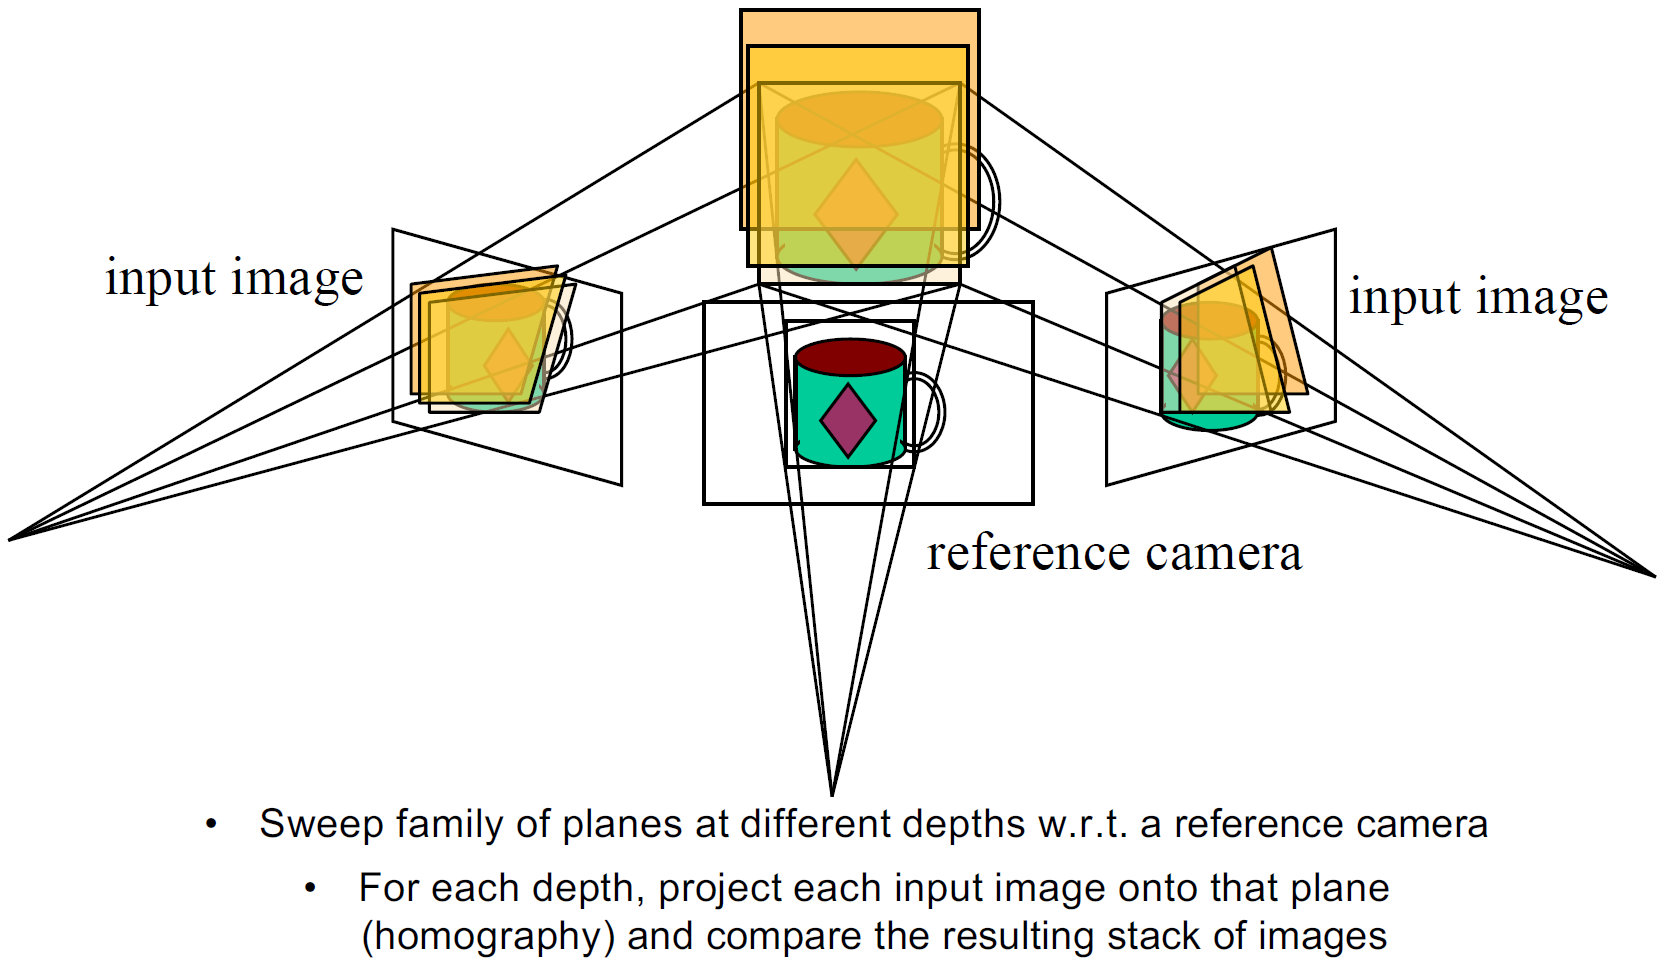
\includegraphics[width=1\columnwidth]{figures/plane-sweep-volume.png}
    \caption{Plane Sweep Volume Representation~\cite{svetlana_2019}}
    \label{fig:plane-sweep-volume}
\end{figure}

Collins~\cite{collins_space-sweep_1996} applied the PSV representation to the problem of reconstructing the 3D scene from multiple views while simultaneously performing feature matching across all views sharing common features. Feature matching is the process of matching corresponding ``features of interest" characterized by their repeatability across multiple views of the same world scene. Examples include keypoints, corners, edges, objects, etc. Matched views can be rectified and used for triangulating depth, etc., as mentioned in section~\ref{sec:motivation}. In the author's implementation, instead of going for a resource-intensive 3D representation that would require splitting the entire 3D scene space into voxels and reprojecting\footnote{projecting to a target plane by unapplying and applying the homographies needed to project to the source and target planes, respectively, while accounting for surface normals, plane offsets, camera rotations and translations, etc., as described in subsection~\ref{subsec:base-papers}} all feature points from all views in such manner that the reprojected light rays passed through this uniformly partitioned space, he sampled the 3D scene space at various 2D planes along the depth ($z$) axis, as if capturing just one 2D plane sweeping though it at various instants in time. He partitioned the sweeping plane into cells and allowed each reprojected light ray to vote for a group of cells that fell within a certain radius of the point of intersection of the light ray with the plane. This accounts for the fact that rays from corresponding feature points across all views may not converge most of the time due to reprojection errors. He then chose the $z$-coordinate of the sampled plane containing the cell with the maximum votes for a feature point to be the $z$-coordinate of the feature point in the world scene. The $x$ and $y$ world coordinates would be defined by this winning cell. The victor cell would also determine the 2D feature point correspondences simultaneously just by virtue of the converging rays being retraced to their respective originating views. PSVs, in their various reimplemented forms, have become almost synonymous of layered volumetric representations these days (Figure~\ref{fig:plane-sweep-volume}).

Shade et al.'s~\cite{shade_layered_1998} Layered Depth Image (LDI) scene representation is similar to MPI scene representation in that both MPI and LDI consist of a series of fronto-parallel planes facing a chosen reference viewpoint and placed at varying depths from it. These planes contain the RGB information of the original pixels of the scene's image(s), segregated according to depth. MPI differs from LDI (and PSV) in that it has alpha masking effects at each layer, as it is generated with alpha transparency maps for each layer. Also, MPIs have fixed depths for each layer as opposed to the variable layer depths of LDIs (and PSVs). But in both cases, by virtue of layering, users are able to experience a simulation of what happens when they move their heads while looking at a scene in the world --- they are able to look around foreground objects that occlude background ones. 

Szeliski and Golland~\cite{szeliski_stereo_1999} first introduced the MPI representation for purposes of stereo matching with simultaneous RGBA estimation at each matched pixel. Stereo matching, otherwise called disparity mapping, uses feature matching techniques such as SIFT\footnote{Scale-Invariant Feature Transform~\cite{lowe_distinctive_2004}} in pixel-and-sub-pixel-wise disparity estimation for 3D scene reconstruction from rectified stereo images. The authors' framework was the first to extract high-accuracy depth, color, and transparency maps for several images at a time, operating even at sub-pixel levels. They were able to enforce sub-pixel accuracy and perform effective matte separation of foreground and background elements despite the usual 3D vision challenges such as occlusions, etc., because they came as close to modern ML reimplementations as possible. They implemented various loss functions such as a pixel-wise weighted photometric $L_1$ norm between the input and reprojected images, a per-pixel smoothness constraint on the RGBA values allowed in the reprojected images, etc. They then performed an iterative refinement of the estimated RGBA values with the help of a gradient\footnote{vector of partial derivatives of the function(s) to be optimized} descent algorithm designed to optimize a combination of all these losses, but sans the explosive power of neural networks.

\subsection{Influential Work}\label{subsec:influential-work}

DeepStereo~\cite{deep_stereo_2016} was the first to apply CNNs in an end-to-end manner to novel view synthesis from diverse collections of indoor and outdoor imagery in the wild, given the availability of camera parameters\footnote{camera intrinscics such as focal length and principal point and camera extrinsics/pose such as position and orientation} for each input image. Their paper describes why it would be unwise to expect a typical present-day CNN to synthesize any ground-truth target image without being provided with the pose of the view as well --- the network would needlessly be learning epipolar geometry itself! Epipolar geometry --- the geometry of binocular and multi-view stereo vision --- gives us the epipolar constraint $x'^T F x = 0$ between all corresponding points $x$ and $x'$ on a stereo pair. Here, $F$ is called the fundamental matrix and is derived from the intrinsic and extrinsic parameters of the stereo cameras involved. To circumvent such an indeterminable and expensive pixel-to-pixel training scenario, the authors had PSVs (Figure~\ref{fig:plane-sweep-volume}) come to the rescue. They supplied all input views required to synthesize a target view as separate PSVs to their network. Each input plane sweep would contain all pixels of the respective input view reprojected onto a chosen number of planes at chosen depths in the usual ``stack of acetates" manner, with the planes all having their viewpoints match with the target view's. The plane that each RGB pixel gets reprojected onto will also determine the availability of the pixel (as alpha values ranging from 0 to 1) to the surrounding voxels of the PSV. The plane sweep of each input view has the pose information of the view implicitly encoded in it just by virtue of its construction. Moreover, the plane sweeps of all input views of the same scene trivially enforce the epipolar constraint as all matching pixels across these originating input views may be located in the same depth-wise column of each plane sweep. Each of these depth-wise columns may then be computed upon by the network independently of other columns, in producing the corresponding synthesized target pixel. The network learns to predict the best weight and color for each reprojected pixel on all input planes, so it may perform a weighted summation of these estimated pixel colors and obtain a final predicted target pixel color. Such averaging has a smoothing effect over the color values of the synthesized target image. The error signal that is iteratively minimized by the training is given by the pixel-wise $L_1$ (absolute difference) loss between the actual target color $C_{i,j}^t$ and the synthesized target color $C_{i,j}^s$ at each pixel $(i,j)$:

\[\mathcal{L} = \sum_{i,j} |C_{i,j}^t - C_{i,j}^s|\]

Kalantari et al.'s~\cite{kalantari_2016} model learns to interpolate novel views in the 8x8 central view grid of a Lytro camera containing a microlens array. It was the state-of-the-art learning-based view synthesis model prior to Zhou et al.'s~\cite{zhou2018stereo} \textit{stereo magnification} MPI model. It is composed of disparity and color predictor components in the form of simple 4-layered sequential CNNs. The training signal it optimizes is given by the $L_2$ (squared difference) pixel reconstruction loss between each pair of original and interpolated target views.

Both DeepStereo and Kalantari et al. are unable to train on training images in their entirety. Instead, they extract patches of training images for their models to train on. This is because, unlike how Zhou et al.'s model is designed to predict a global scene representation once for a pair of views belonging to the same scene and render many novel views with it at near-real-time speeds, the former models are designed to predict each novel view in an end-to-end fashion independently of other novel views and so have to rerun their prediction pipelines every time, making novel view synthesis prohibitively slow for high-resolution and real-time applications. Moreover, when rendering nearby views, the former methods produce much more artifact-ridden, spatially-incoherent views compared to the views inferred by Zhou et al. What Zhou et al. has going for it in these scenarios is an implicit smoothness prior imposed by the common scene representation over the color and depth values being inferred for each synthesized nearby view. 

What also comes close to the MPI representation is the layered representation of Penner and Zhang~\cite{penner_soft_2017}. But then again, in all these prior methods, a unique scene representation is predicted in the reference coordinate frame of each target view to be rerendered, negatively impacting view synthesis efficiency. Other innovative MPI-related papers released subsequently to Zhou et al. and leading up to Tucker and Snavely's~\cite{single_view_mpi} \textit{single-view} MPIs are 2019's Srinivasan et al.~\cite{srinivasan_pushing_2019}, Mildenhall et al.~\cite{mildenhall_local_2019}, and DeepView~\cite{flynn_deepview_2019}. Srinivasan et al. improved the quality and increased the disparity and baseline ranges of predicted MPIs and rendered views, by bringing in a 3D CNN architecture, training on random-resolution views, and introducing an optical flow constraint over the appearance of occluded content in rendered views. Mildenhall et al.'s model converts an grid of irregularly sampled views into MPIs, i.e., mini-light-field representations, and blends such nearby local light fields to render novel views. They were able to establish a minimum density of sampled views required for robust rendering, which turned out to be 4000$\times$ less than the Nyquist frequency required to prevent aliasing. DeepView~\cite{flynn_deepview_2019} replaced the update step\footnote{involving step size and other parameters such as priors/biases} of the network's gradient descent algorithm with a CNN that learns the various gradient descent parameters instead. As a consequence, the network takes much larger strides along the direction of optimization and converges much sooner and with more accuracy than a network using standard gradient descent. However, these methods do not tackle the monocular-image approach for generating MPIs.

\subsection{Base Papers}\label{subsec:base-papers}

Zhou et al.~\cite{zhou2018stereo} was the first to implement view extrapolation to significantly larger baselines (up to 8$\times$ input baselines) than prior work --- a process they call stereo magnification. They use stereo pairs to learn an MPI (Figure~\ref{fig:mpi-layered-representation}) prediction network in the following manner:

\begin{figure}[!h]
    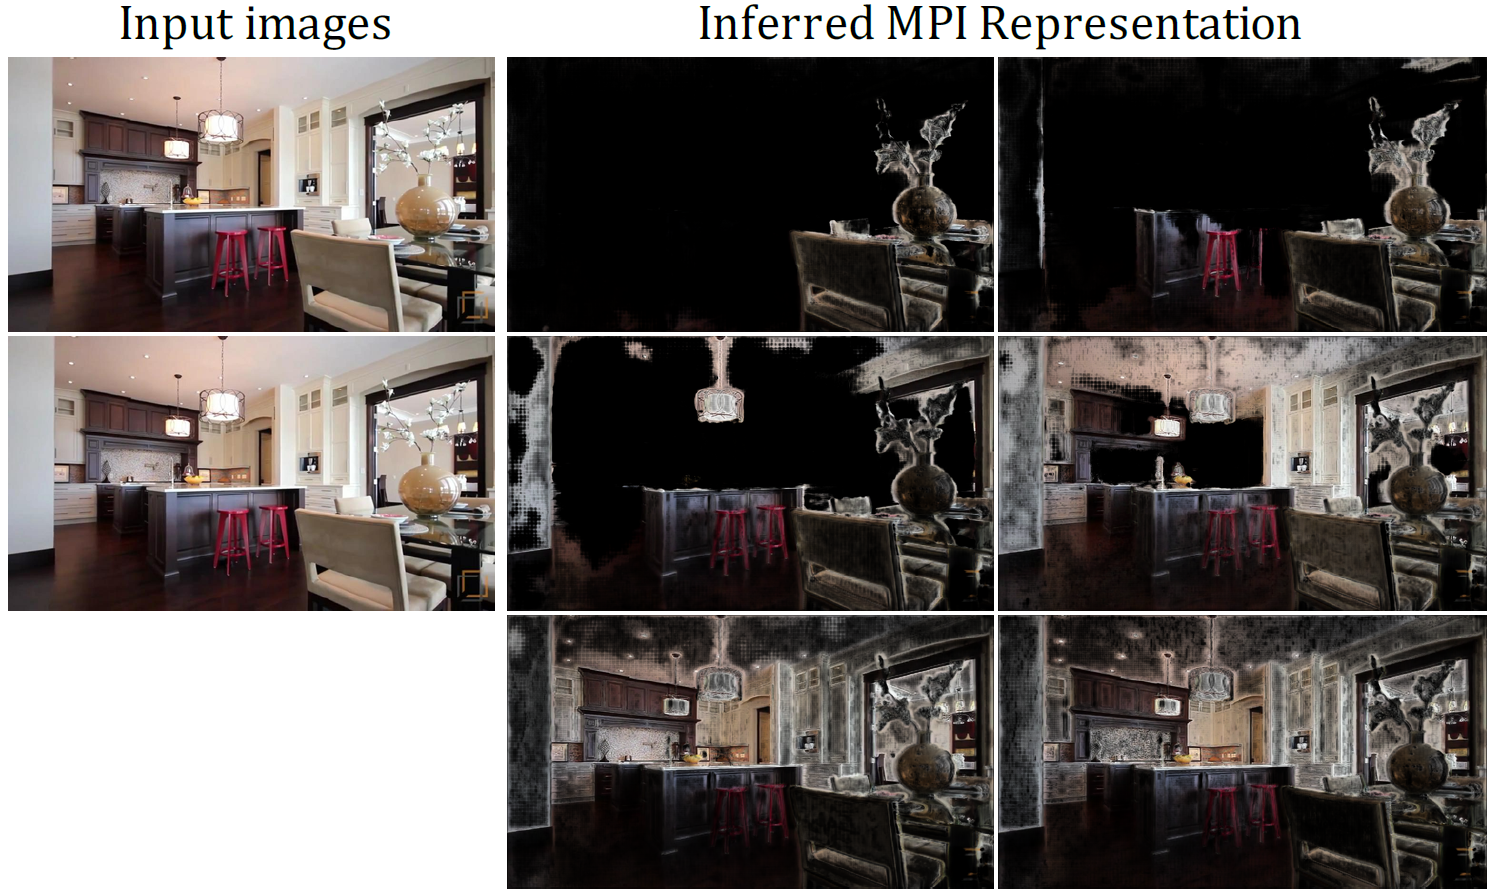
\includegraphics[width=0.75\columnwidth]{figures/inferred-mpi.png}
    \caption{Inferred MPI~\cite{zhou2018stereo}}
    \label{fig:inferred-mpi}
\end{figure}

\begin{itemize}
    \item The camera parameters $c_1 = (p_1,\ k_1)$ and $c_2 = (p_2,\ k_2)$ of the stereo pair, $(I_1,\ I_2)$, are also needed for the prediction process, along with the target image $I_t$ and its parameters $c_t$. Here, $p$'s and $k$'s refer to the camera extrinsics and intrinsics of the respective images.
    \item The viewpoint of one image of the stereo pair, $I_1$, is used as the reference viewpoint for the MPI to be predicted at. Hence, $p_1$ would be the identity pose $[I|\boldsymbol{\mathit{0}}]$.
    \item The goal is to learn a network that generates an MPI representation (Figure~\ref{fig:inferred-mpi}) with inputs $(I_1,\ I_2,\ c_1,\ c_2)$ such that when the MPI is rendered at viewpoint $c_t$, it would produce the target image $I_t$. 
    \item As demonstrated by DeepStereo~\cite{deep_stereo_2016}, an effective way to encode pose information for training is via a PSV (Figure~\ref{fig:plane-sweep-volume}). Hence, the input to their customized encoder-decoder type network includes a PSV version of $I_2$ $(\hat{I_2})$ with the planes all reprojected into the output MPI's viewpoint, $c_1$, and with the entire plane sweep concatenated internally and with an unaltered $I_1$ along the three color channels. The depth planes of $\hat{I_2}$ are also chosen to coincide with the ones of the output MPI.
    \item The 3D structure of the scene depicted by $I_1$ and $I_2$ is automatically learnt by the network by merely being able to compare $I_1$ with each of the reprojected images of $I_2$ in the input stack $(\hat{I_2^1},\ \hat{I_2^2},\ \ldots,\ \hat{I_2^D},\  I_1)$, where $D$ is the total number of MPI depth planes. The depth at each pixel of any known or novel view of the scene must be the depth of the plane where $I_1$ and $\hat{I_2}$ concur.
    \item In order to reduce resource consumption due to network over-parameterization, the network's initial outputs do not consist of separate RGBA maps for each MPI layer but rather just a ``background" image intended to capture pixels occluded in $I_1$ and a set of color blending weight maps and alpha maps for each MPI layer.
    \item The actual RGB values in each layer, $C_i$, are then easily computed by taking the per-pixel weighted average of $I_1$ and the predicted background image $\hat{I_b}$:
    
    \[C_i = w_i \odot I_1 + (1 - w_i) \odot \hat{I_b}\]
    
    Here, $\odot$ is the Hadamard product and $w_i$ refers to the RGB blending weights from the initial network output, specific to MPI layer $i$.
    \item $\hat{I_b}$ need not itself be a natural image as the network can selectively and softly blend each $\hat{I_b}$ pixel with $I_1$, based on respective layer $\alpha$'s and $w$'s. Intuitively, $I_1$'s contribution would be more in foreground layers than in the background ones; and conversely for $\hat{I_b}$. 
\end{itemize}

The rest of the training pipeline consists of the rendering of the MPI at the target viewpoint, $c_t$, and the gradient descent algorithm involving a VGG perceptual (similar to LPIPS~\cite{zhang_unreasonable_2018}) loss function between the rendered view and ground-truth target view. The perceptual loss is proven to be more robust than unmodified pixel reconstruction losses such as $L_1$ and $L_2$ norms. Adam gradient descent algorithm is used (similarly to Tucker and Snavely~\cite{single_view_mpi}) to optimize this loss. Adam~\cite{kingma_adam_2017} is better than regular stochastic gradient descent but is still not superior to DeepView's~\cite{flynn_deepview_2019} implementation of learned gradient descent. Rendering an MPI first involves warping each RGBA MPI layer onto the target camera's image plane using the standard inverse homography or reprojection operation~\cite{hartley_multiple_2004}, as illustrated in figure~\ref{fig:standard-inverse-homography}. But, anticipating usual reprojection mismatches, they resample each pixel to be warped by bilinear interpolation with respective four-grid neighbors. These rerendered MPI layers are then alpha-composited in back-to-front order to get the final predicted target view. All elements of the rendering process are differentiable.

\begin{figure}[!h]
    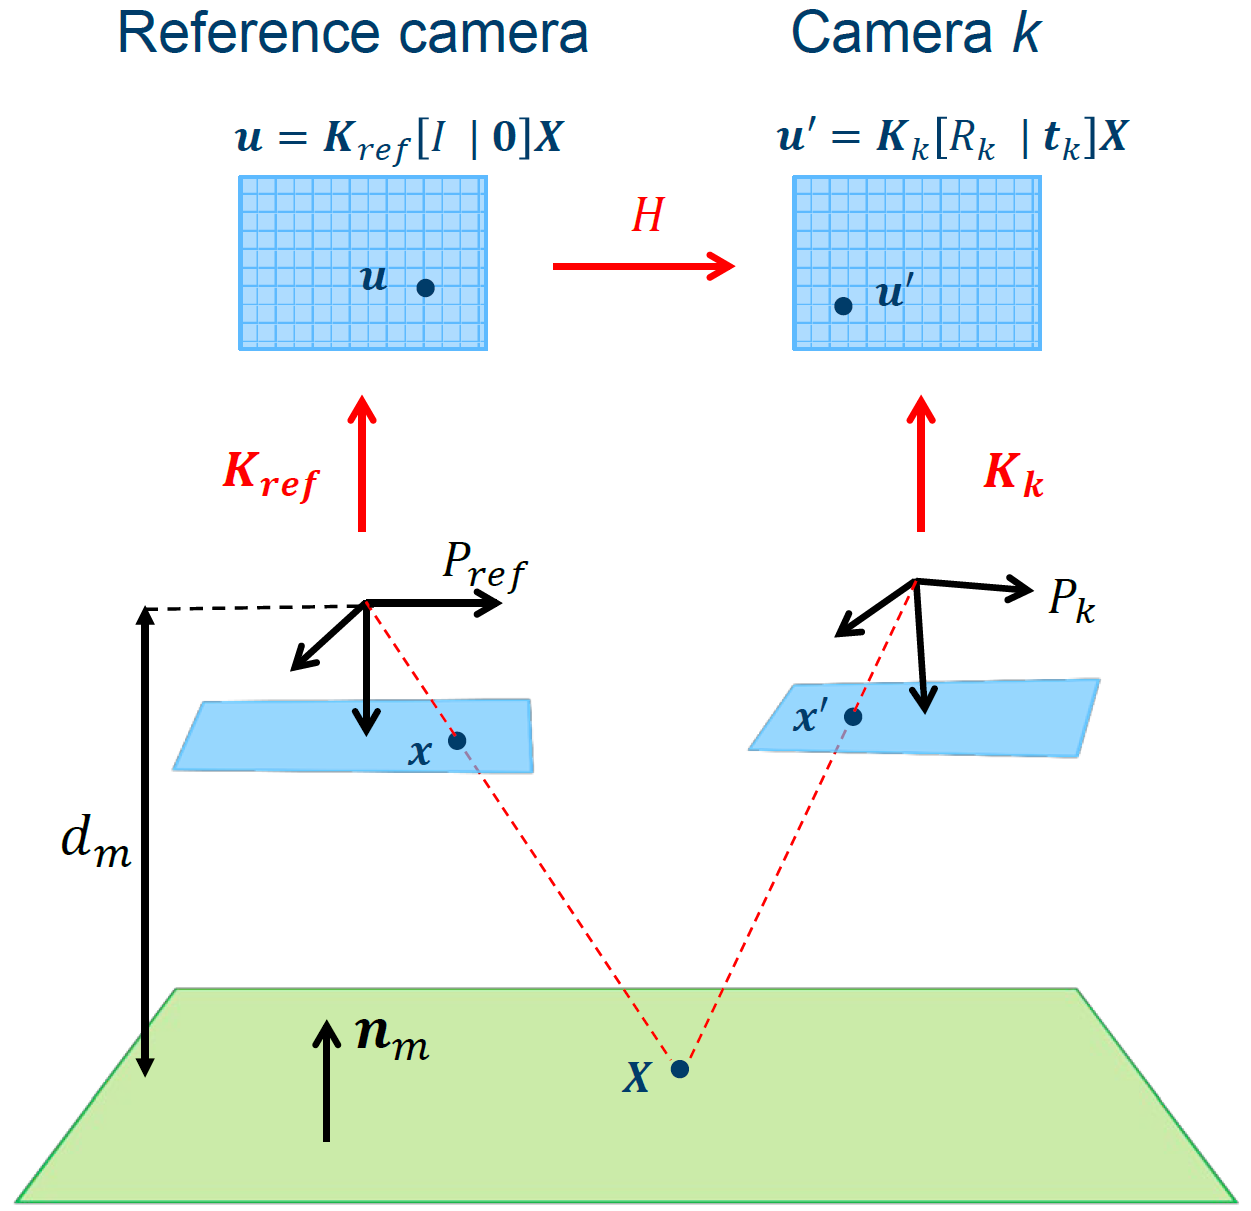
\includegraphics[width=0.75\columnwidth]{figures/standard-inverse-homography.png}
    \caption{Standard Inverse Homography or Reprojection~\cite{brann_forelesninger_2016}}
    \label{fig:standard-inverse-homography}
    {\small Here, the 3D point $\boldsymbol{X}$ on the MPI plane in the world is the \textit{homogeneous} version (determined up to scale) of its projection $\boldsymbol{x}$ on the reference camera's image plane in camera coordinates, i.e., with the camera's image plane centered at the camera center, $c_{ref}$. More precisely, $\boldsymbol{X} = [X,Y,d_m]^T \sim \tilde{\boldsymbol{x}} = [X/d_m,Y/d_m,1]$. This is because all MPI world planes are fronto-parallel to the reference camera and their equations can be given by $\boldsymbol{n_m \cdot \tilde{x}} + a = 0$, where $\boldsymbol{n_m} = [0,0,1]$ is the plane normal and $a = -d_m$ is the plane offset from $c_{ref}$. The projection $\boldsymbol{u}$ on the reference camera's image plane in regular image coordinates is attained by applying reference camera intrinsics $\boldsymbol{K_{ref}}$ to $\boldsymbol{x}$. Since the MPI is not necessarily fronto-parallel to the target camera $c_k$, $\tilde{\boldsymbol{x'}}$ need not be $[X/d_m,Y/d_m,1]$ even though $\boldsymbol{X} \sim \tilde{\boldsymbol{x'}}$ as well. $\boldsymbol{u'}$ and $\boldsymbol{K_k}$ similarly belong to the target camera, as does target camera pose (relative to reference camera) $[R_k|\boldsymbol{t_k}]$. The world plane \textit{induces} the homography $H = \boldsymbol{K_k} (R_k - \boldsymbol{t_k} \boldsymbol{n_m}^T / a) \boldsymbol{K_{ref}}^{-1}$ between the image planes of $c_{ref}$ and $c_k$, so we can go from $\boldsymbol{u}$ to $\boldsymbol{u'}$. To go from $\boldsymbol{u'}$ back to $\boldsymbol{u}$, we'd use $H^{-1}$~\cite{zikuicai_derivation_2019}.}  
\end{figure}

Zhou et al.'s methods are ingenious in a number of ways. They trained their model to predict novel views at varying distances from input views so as not to overfit to predicting only up to a limited number of baselines. They used assorted but apt convolutional layers such as dilated convolutions to bring back larger scene contexts at lower computational costs and fractionally-strided convolutions~\cite{prove_introduction_2018} with skip connections~\cite{adaloglou_intuitive_2020} from preceding layers to capture even the finer texture details. The use of VGG perceptual loss allowed them to retain these intricate micro textures together with macro object geometries in synthesized views. Also commendable is their meticulous RealEstate10K dataset creation process which was continued by Tucker and Snavely~\cite{single_view_mpi} in bringing the dataset to it's current state~\cite{zhou2018stereo}. Knowing that state-of-the-art Structure from Motion (SfM) and bundle adjustment\footnote{initial scene reconstruction, camera calibration (including field of view estimation), and pose estimation for a candidate pair of scene views, followed by simultaneous iterative refinement of the 3D scene structure and all estimated camera parameters, using each additional view of the scene, as well, for feature matching} algorithms such as COLMAP~\cite{schoenberger2016sfm,schoenberger2016mvs} are not yet fully optimized for camera tracking in videos, they first subject candidate real estate YouTube videos to Simultaneous Localization And Mapping (SLAM) techniques such as ORB-SLAM2~\cite{mur-artal_orb-slam_2015} to obtain initial camera parameter estimates for all consecutive frames tracked. Consecutive, here, implies that each tracked frame's viewpoint is no farther than a certain percentage of the average of its two neighboring viewpoints. This process naturally breaks a video apart into clips with smoother camera motion. They then process all video clips obtained this way with COLMAP to get a sparse 3D point cloud reconstruction of the scene in each clip and a refined set of camera parameter estimates for all frames. As a final step, they \textit{scale-normalize} each subsequence and its reconstructed camera parameters and 3D points in one shot by scaling the point cloud up or down so the nearest set of points is at a fixed distance from the cameras. Points clouds are discarded by Zhou et al. after scale-normalizing the dataset whereas they are used by Tucker and Snavely~\cite{single_view_mpi} to ``scale-normalize", effectively, their entire single-view training process itself, for they don't have the luxury of inferring parameter and scene scale from more than one view at a time like how Zhou et al. does. SfM involves the estimation of the (generally sparse) 3D structure of a static scene from the multiple (usually unstructured) views of a (often uncalibrated) camera moving around the scene, accompanied by the simultaneous estimation of respective camera parameters. It is essentially a more generic version of Multi-View Stereo (MVS), which itself is an extension of stereo matching and requires known camera parameters to reconstruct (mostly) dense 3D points clouds. COLMAP is capable of both SfM and MVS. Both SfM and MVS can utilize bundle adjustment similarly to SLAM from the Robotics community. SLAM doesn't stop at bundle adjustment but rather proceeds to map out the entire terrain encountered by a robot by making connections between camera trajectories, viewed scenes, etc.~\cite{noauthor_what_nodate}. 

Zhou et al. made some major observations in their various ablation studies. They found that their model trained better on their preferred MPI prediction format consisting of a predicted background image that is blended with the reference image (taken as foreground) using a set of predicted color blending weights, to form each layer of the MPI. This format beat other, more-expressive formats such as ones with an additional predicted foreground or with fully predicted MPI layers. They speculate that the network's somewhat diminished performance with the latter formats could be because of network over-parameterization, more utilization of synthesized layers rather than the original reference image, and perhaps even because of lesser camera movement between the synthesized layers for the network to efficiently learn depth complexity out of. Moreover, they were able to verify that the greater the number of MPI planes used, the higher would be the model's training performance and the quality of synthesized views. Their model presents considerable scope for improvement when it comes to accurately localizing and fixing the depths of multiple overlapping fine textures, avoiding ``stacks of cards" edges in synthesized views when the disparity between the neighboring layers of an MPI exceeds one pixel, etc.

Tucker and Snavely~\cite{single_view_mpi} was the first to implement learning-based single-view view synthesis on videos in the wild. It is fascinating to see how they were able to achieve efficient single-view view synthesis --- an objective coveted by Vision and Graphics communities. Moreover, there are numerous other perks to their model. It produces byproduct disparity maps that can be used in imposing a smoothness prior over synthesized viefws, in computing a global scale factor, etc. It learns to inpaint occluded content behind foreground objects without requiring ground truth 3D or depth, mainly due to their utilization of \textit{scale-invariant} view synthesis for supervision. As mentioned previously in this subsection, although Tucker and Snavely extended RealEstate10K dataset by adopting the same methods as Zhou et al.~\cite{zhou2018stereo}, yet they had to incorporate scale-normalization/scale-invariance into their training in order to circumvent the global scale factor ambiguity that arises when attempting to infer scene geometry from monocular views. They accomplish this in the following manner (Figure~\ref{fig:tucker-snavely-pipeline}):

\begin{figure}[!h]
    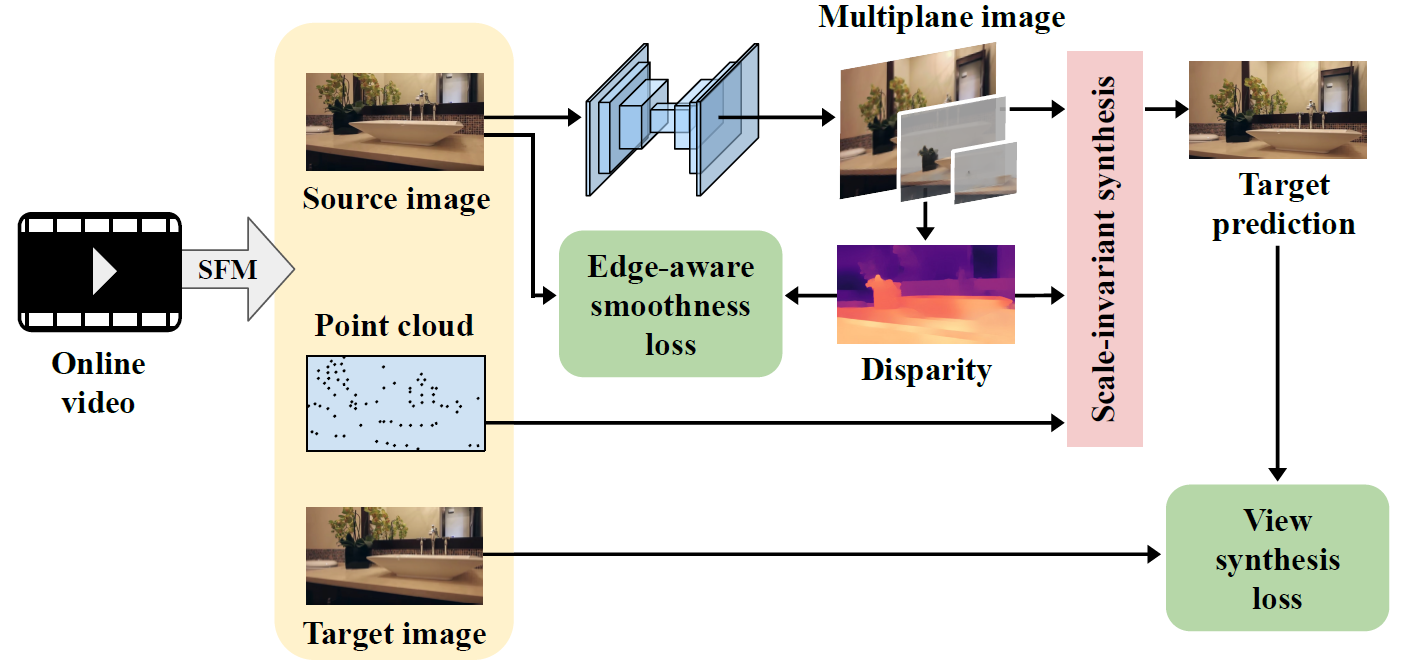
\includegraphics[width=1\columnwidth]{figures/tucker-snavely-pipeline.png}
    \caption{Tucker and Snavely's Single-View View Synthesis Pipeline~\cite{single_view_mpi}}
    \label{fig:tucker-snavely-pipeline}
\end{figure}

\begin{itemize}
    \item The sparse point cloud of the scene depicted by each group of sequential video frames, the lists of all 3D points \textit{visible} from each frame, the camera parameters of each frame, and the video frames themselves are needed for training. All these input components result from the ORB-SLAM2, COLMAP, and scale-normalization procedures of Zhou et al.
    \item Pairs of source and target frames $(I_s,\ I_t)$ and respective camera parameters $(c_s,\ c_t)$ are randomly picked for training, along with the respective visible point sets of source frames. The sets of visible points are converted from world coordinates to camera coordinates to get a final point set $P_s = \{(x,\ y,\ d),\ \ldots\}$ for each source frame, where the $z$-coordinate of each world point becomes the depth $d$ of the world point from the source camera, and the mapped 2D points are denoted by the positions $(x,\ y)$ within the source image. 
    \item Similarly to Zhou et al., Tucker and Snavely's chosen reference camera for the MPI planes (Figure~\ref{fig:mpi-layered-representation}) is $c_s$, and their preferred MPI prediction format consists of a predicted background image $\hat{I_b}$, a set of layer-wise predicted alphas, and a set of layer-wise color blending weights that (unlike Zhou et al.) are calculated from the alphas and not predicted by the network. Tucker and Snavely derives color blending weights $w_i$ for each MPI layer $i$ as $w_i = \underbrace{\prod_{j>i} (1 - \alpha_j)}$, and final color values $C_i$ for each layer as $C_i = w_i I_s + (1 - w_i) \hat{I_b}$.
    \item Similarly to Zhou et al., when rendering an MPI, Tucker and Snavely's warping function $\mathcal{W}$ uses bilinear sampling and standard inverse homography (Figure~\ref{fig:standard-inverse-homography}) to warp each layer from source viewpoint $c_s$ to target viewpoint $c_t$: $C_i' = \mathcal{W}_{c_s, c_t}(\sigma d_i, C_i)$; $\alpha_i' = \mathcal{W}_{c_s, c_t}(\sigma d_i, \alpha_i)$. The only difference is that Tucker and Snavely's $\mathcal{W}$ scales the depths by a factor $\sigma$, which they compute separately for each training instance.
    \item To get the final rerendered target $\hat{I_t}$, the warped layers $(C_i', \alpha_i')$ are alpha-composited as usual: $\hat{I_t} = \sum_{i=1}^D \left(C_i' \alpha_i'\ \underbrace{\prod_{j=i+1}^D (1 - \alpha_j')}\right)$. Besides, the disparity map $\hat{D_s}$ of the source image can also be similarly synthesized from the MPI using the inverse depths $d^{-1}$ of visible points $P_s$: $\hat{D_s} = \sum_{i=1}^D \left(d_i^{-1} \alpha_i\ \underbrace{\prod_{j=i+1}^D (1 - \alpha_j)}\right)$.
    \item DeepView~\cite{flynn_deepview_2019} describes the under-braced terms in all previously mentioned formulae to be the \textit{net transmittance} at respective depth planes $i$. They reason that the terms represent the fraction of the color/disparity that persists in layer $i$ after getting attenuated through all prior layers.
    \item Learning the 3D scene structure from a single view is trickier than from multiple views, for only the relative pose between multiple views can implicitly resolve global scale ambiguity. But Tucker and Snavely's method is able to accept source and target inputs of unknown scale and still make rerendered images match ground-truth because they solve for the unknown scale factor as part of their MPI generation. They observe that RealEstate10K-dataset-derived inputs $c_s$, $c_t$, and $P_s$ are consistent in scale for each training instance. They, therefore, compute $\sigma$ to be the scale factor that minimizes the log-squared error between the predicted disparity map $\hat{D_s}$, bilinearly sampled at each position $(x,y)$, and the point set $P_s$:
    
    \[\sigma = exp \left[\frac{1}{|P_s|} \sum_{(x,y,d) \in P_s} (ln \hat{D_s}(x,y) - ln(d^{-1}))\right]\]
    
    After $\sigma$ is applied in warping with $\mathcal{W}$ as shown before, the rendered image no longer varies with the scale of the input viewpoints and point set, and can be used in the various loss functions. 
    \item Their weighted aggregate loss function is given by
    
    \[\mathcal{L} = \lambda_p \mathcal{L}^{pixel} + \lambda_s \mathcal{L}^{smooth} + \lambda_d \mathcal{L}^{depth}\]
    
    Here, $\mathcal{L}^{pixel}$ is just the regular $L_1$ photometric distance between synthesize and ground-truth target views:
    
    \[\mathcal{L}^{pixel} = \sum_{channels} \frac{1}{N} \sum_{(x,y)} |\hat{I_t} - I_t|\]
    
    $\mathcal{L}^{smooth}$ is the \textit{edge-aware smoothness loss} that prevents the gradients of the synthesized disparity map $\hat{D_s}$ from crossing a certain threshold ($g_{min}$, usually 0.05) whenever there is no edge detected in the source image, like so: 
    
    \[\mathcal{L}^{smooth} = \frac{1}{N} \sum_{(x,y)} \left(max\left(G(\hat{D_s}) - g_{min},\ 0\right) \odot (1 - E_s)\right)\]
    
    where $\odot$ is the Hadamard product, $G$ represents the $L_1$ norm of the gradient of an image summed over all three color channels, like so:
    
    \[G(I) = \sum_{channels} ||\nabla I||_1\]
    
    where Sobel filters are used to compute the gradient, and $E_s$ represents a custom edge detector for the source image, which signals the presence of an edge whenever the gradient of the source image is at least a fraction ($e_{min}$, usually 0.1) of its own maximum value over the entire image, like so:
    
    \[E_s = min \left(\frac{G(I_s)}{e_{min} \times max_{(x,y)} G(I_s)},\ 1\right)\]
    
    and $\mathcal{L}^{depth}$ is a sparse depth loss given by the $L_2$ difference between the logs of the disparities derived using the predicted alphas (i.e., the synthesized disparity map) on the on hand and the input point set $P_s$ and the other, like so
    
    \[\mathcal{L}^{depth} = \frac{1}{|P_s|} \sum_{(x,y,d) \in P_s} \left(ln\frac{\hat{D_s}(x,y)}{\sigma} - ln(d^{-1})\right)^2\]
    
    where the computed scale factor $\sigma$ that minimizes $\mathcal{L}^{depth}$ is itself included.
\end{itemize}

The network used is architecturally similar to DispNet~\cite{mayer_large_2016}. In our work, in the process of recreating Tucker and Snavely's model and retraining it on video-chat-relevant scenes, we have reimplemented their weighted aggregate loss function, among other model features. We retained their chosen loss function weights of $\lambda_p = 1$, $\lambda_s = 0.5$, and $\lambda_d = 0.1$. We also retained their choice of optimizer --- Adam --- with learning rate 0.0001.

Even though there is still a lot of scope for improvement in performance with regard to model-induced artifacts reducing the quality of synthesized views, Tucker and Snavely's authors share how the various aspects of the model contribute to it beating the state-of-the-art. They show that the scale-invariant nature of the model's supervision by view synthesis (i.e., usage of ground-truth target views) plays a major role in its success, followed by the edge-aware smoothness prior, and the chosen MPI format involving a predicted background. Another triumph of their model is that even though it does not use depth supervision at all, it is comparable to state-of-the-art depth prediction methods that use explicit depth supervision. Their project presents exciting future opportunities such as turning the model into a Generative Adversarial Network (GAN)~\cite{goodfellow_generative_2014} to possibly produce more extensive and realistic inpainting, and so on.